%!TEX root = ../../main.tex


\begin{figure}[!htb]
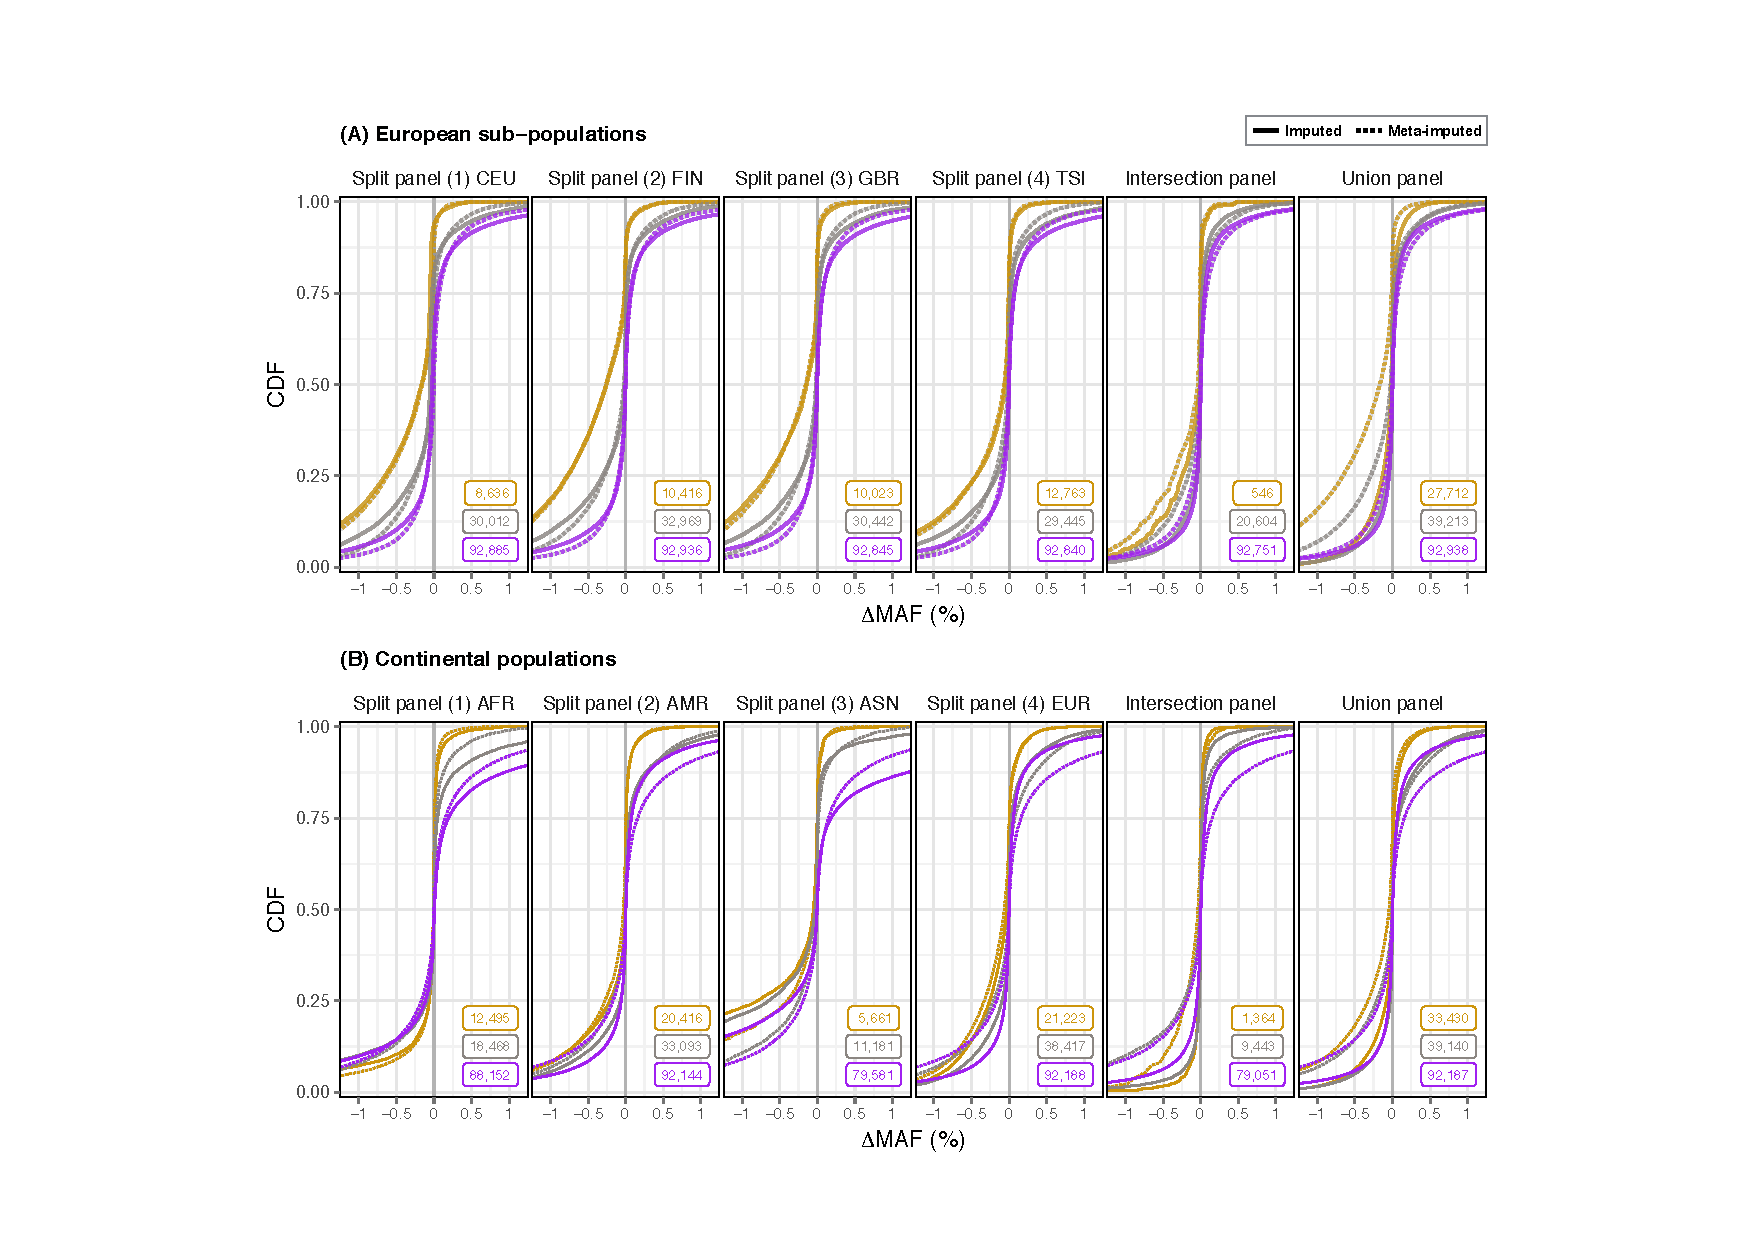
\includegraphics[width=\textwidth]{./img/ch2/accuracy_imputed_delta}
\Caption{Difference between imputed and masked minor allele frequency}
{Comparison of imputed and meta-imputed \gls{maf} in relation to known population frequencies, compared on the same set as retained after \gls{qc} in each comparison.
Frequency difference, ${\Delta\text{MAF}}$, was calculated as the \gls{maf} observed at a masked variant minus \gls{maf} at the corresponding (meta-)imputed variant, pooled in \n{3} \gls{maf} bins; rare variants (${\text{MAF} \in \left[ 0.00, 0.01\right]}$; \emph{yellow}), low-frequency (${\text{MAF} \in \left( 0.01, 0.05\right]}$; \emph{grey}), and common variants (${\text{MAF} \in \left( 0.05, 0.50\right]}$; \emph{purple}).
Numbers per \gls{maf} bin per comparison are given in each panel (\emph{colour-coded}).}
{fig:imp_delta}
\end{figure}
